\documentclass[a4paper,14pt,oneside,openany]{memoir}

\usepackage{geometry}
\usepackage{comment}
\usepackage{totcount} %counter

%%% Математические пакеты %%%
\usepackage{amsthm,amsmath,amscd}   % Математические дополнения от AMS
\usepackage{amsfonts,amssymb}       % Математические дополнения от AMS
\usepackage{mathtools}              % Добавляет окружение multlined
\usepackage{xfrac}                  % Красивые дроби
\usepackage[
locale = DE,
list-separator       = {;\,},
list-final-separator = {;\,},
list-pair-separator  = {;\,},
list-units           = single,
range-units          = single,
range-phrase={\text{\ensuremath{-}}},
% quotient-mode        = fraction, % красивые дроби могут не соответствовать ГОСТ
fraction-function    = \sfrac,
separate-uncertainty,
]{siunitx}[=v2]                 % Размерности SI
\sisetup{inter-unit-product = \ensuremath{{}\cdot{}}}


%TODO???
%\usepackage[plain]{algorithm}
\usepackage[linesnumbered,ruled,vlined]{algorithm2e}
%%% Coloring the comment as blue
\newcommand\mycommfont[1]{\footnotesize\ttfamily\textcolor{blue}{#1}}
\SetCommentSty{mycommfont}
\SetKwInput{KwInput}{Input}                % Set the Input
\SetKwInput{KwOutput}{Output}              % set the Output
%end----algorithm2e

%TODO???
\usepackage{listings} %Inserting code in this LaTeX document
\usepackage{matlab-prettifier} %https://www.overleaf.com/learn/latex/Questions/How_can_I_include_MATLAB_code_in_my_LaTeX_document%3F
%решаем проблему с кириллицей в комментариях (в pdflatex) https://tex.stackexchange.com/a/103712
\lstset{extendedchars=true,keepspaces=true,literate={Ö}{{\"O}}1
	{Ä}{{\"A}}1
	{Ü}{{\"U}}1
	{ß}{{\ss}}1
	{ü}{{\"u}}1
	{ä}{{\"a}}1
	{ö}{{\"o}}1
	{~}{{\textasciitilde}}1
	{а}{{\selectfont\char224}}1
	{б}{{\selectfont\char225}}1
	{в}{{\selectfont\char226}}1
	{г}{{\selectfont\char227}}1
	{д}{{\selectfont\char228}}1
	{е}{{\selectfont\char229}}1
	{ё}{{\"e}}1
	{ж}{{\selectfont\char230}}1
	{з}{{\selectfont\char231}}1
	{и}{{\selectfont\char232}}1
	{й}{{\selectfont\char233}}1
	{к}{{\selectfont\char234}}1
	{л}{{\selectfont\char235}}1
	{м}{{\selectfont\char236}}1
	{н}{{\selectfont\char237}}1
	{о}{{\selectfont\char238}}1
	{п}{{\selectfont\char239}}1
	{р}{{\selectfont\char240}}1
	{с}{{\selectfont\char241}}1
	{т}{{\selectfont\char242}}1
	{у}{{\selectfont\char243}}1
	{ф}{{\selectfont\char244}}1
	{х}{{\selectfont\char245}}1
	{ц}{{\selectfont\char246}}1
	{ч}{{\selectfont\char247}}1
	{ш}{{\selectfont\char248}}1
	{щ}{{\selectfont\char249}}1
	{ъ}{{\selectfont\char250}}1
	{ы}{{\selectfont\char251}}1
	{ь}{{\selectfont\char252}}1
	{э}{{\selectfont\char253}}1
	{ю}{{\selectfont\char254}}1
	{я}{{\selectfont\char255}}1
	{А}{{\selectfont\char192}}1
	{Б}{{\selectfont\char193}}1
	{В}{{\selectfont\char194}}1
	{Г}{{\selectfont\char195}}1
	{Д}{{\selectfont\char196}}1
	{Е}{{\selectfont\char197}}1
	{Ё}{{\"E}}1
	{Ж}{{\selectfont\char198}}1
	{З}{{\selectfont\char199}}1
	{И}{{\selectfont\char200}}1
	{Й}{{\selectfont\char201}}1
	{К}{{\selectfont\char202}}1
	{Л}{{\selectfont\char203}}1
	{М}{{\selectfont\char204}}1
	{Н}{{\selectfont\char205}}1
	{О}{{\selectfont\char206}}1
	{П}{{\selectfont\char207}}1
	{Р}{{\selectfont\char208}}1
	{С}{{\selectfont\char209}}1
	{Т}{{\selectfont\char210}}1
	{У}{{\selectfont\char211}}1
	{Ф}{{\selectfont\char212}}1
	{Х}{{\selectfont\char213}}1
	{Ц}{{\selectfont\char214}}1
	{Ч}{{\selectfont\char215}}1
	{Ш}{{\selectfont\char216}}1
	{Щ}{{\selectfont\char217}}1
	{Ъ}{{\selectfont\char218}}1
	{Ы}{{\selectfont\char219}}1
	{Ь}{{\selectfont\char220}}1
	{Э}{{\selectfont\char221}}1
	{Ю}{{\selectfont\char222}}1
	{Я}{{\selectfont\char223}}1
	{і}{{\selectfont\char105}}1
	{ї}{{\selectfont\char168}}1
	{є}{{\selectfont\char185}}1
	{ґ}{{\selectfont\char160}}1
	{І}{{\selectfont\char73}}1
	{Ї}{{\selectfont\char136}}1
	{Є}{{\selectfont\char153}}1
	{Ґ}{{\selectfont\char128}}1
}


%https://ctan.org/pkg/afterpage 
%– Execute command after the next page break
%- Để sử dụng \afterpage{\clearpage}  thay cho \clearpage??
% cơ bản giống nhau, ko khác gì mấy.
%%% Для добавления Стр. над номерами страниц в оглавлении
%%% http://tex.stackexchange.com/a/306950
%\usepackage{afterpage}

%%% enumitem – Control layout of itemize, enumerate, description
%https://mirror.macomnet.net/pub/CTAN/macros/latex/contrib/enumitem/enumitem.pdf
\usepackage{enumitem}
%To remove the vertical space altogether in all lists: \setlist{nosep}
% A first pattern aligns the label with the surrounding \parindent while the item body is indented depending on the label and a fixed labelsep: labelindent = \parindent, leftmargin = *
\setlist{ %% Каждый пункт, подпункт и перечисление записывают с абзацного отступа (ГОСТ 2.105-95, 4.1.8)
	nosep,
	labelindent=\parindent,
	leftmargin=*
}

%%% Таблицы %%%
\usepackage{longtable,ltcaption} % Длинные таблицы
\usepackage{multirow,makecell}   % Улучшенное форматирование таблиц
\usepackage{tabulary}      % таблицы с автоматически подбирающейся
\usepackage{threeparttable}      % автоматический подгон ширины подписи таблицы

% шириной столбцов (tabu обязательно до hyperref вызывать)
%%% Таблицы %%%
%\DeclareCaptionLabelSeparator{tabsep}{\tablabelsep} % нумерация таблиц
%\DeclareCaptionFormat{split}{\splitformatlabel#1\par\splitformattext#3}

%\usepackage[⟨options⟩]{caption}
\usepackage{caption}                % caption – Customising captions in floating environments https://ctan.org/pkg/subcaption
%https://github.com/kia999/babel-russian/blob/master/russianb.dtx#L958-L967
%2021-01-04 version 1.3m
%* The macro `\cyrdash` that prints Cyrillic dash has been changed.
% Now it is alias of `\textemdash` in all encodings.
%You can define your own caption label separators with\DeclareCaption-
%LabelSeparator \DeclareCaptionLabelSeparator{⟨name⟩}{⟨code⟩}
\DeclareCaptionLabelSeparator{tabsep}{\textemdash} % нумерация таблиц
% \captionsetup[⟨float type⟩]{⟨options⟩}
\captionsetup[table]{
	format=plain,                % формат подписи (plain|hang)
	font=normal,                      % нормальные размер, цвет, стиль шрифта
	skip=.0pt,                        % отбивка под подписью
	parskip=.0pt,                     % отбивка между параграфами подписи
	position=above,                   % положение подписи
	justification=centering, %justified,           % центровка
	indent=0cm,               	 		% смещение строк после первой
	labelsep=tabsep,%endash,                  % thay dấu : thành "--" (ГОСТ 2.105, 4.3.1)
	singlelinecheck=false, % не выравнивать по центру, если умещается в одну строку
}
% Sẽ tự động điều chỉnh bên Figure, ko cần cấu hình lại mỗi lần gọi: \figure
\captionsetup[figure]{
	format=plain,                     % формат подписи (plain|hang)
	font=normal,                      % нормальные размер, цвет, стиль шрифта
	skip=1.5pt,                       % khoảng cách giữa hình và caption. (default=0pt)
	parskip=.0pt,                     % отбивка между параграфами подписи
	position=below,                   % положение подписи
	singlelinecheck=true,             % выравнивание по центру, если умещается в одну строку
	justification=centerlast,         % центровка
	labelsep=tabsep,                  % Sử dụng "--" giống table.
}
%You can define your own caption fonts wit \DeclareCaptionFont{⟨name⟩}{⟨code⟩} .
% e.g. \DeclareCaptionFont{bf}{\bfseries}
%https://mirror.truenetwork.ru/CTAN/macros/latex/contrib/caption/subcaption.pdf
\usepackage{subcaption}             % Support for sub-captions
%\DeclareCaptionSubType[⟨numbering scheme⟩]{⟨type⟩
%%% Подписи подрисунков %%%
\DeclareCaptionSubType{figure} % thêm caption vào hình phụ.
% cấu hình 
\captionsetup[subfloat]{
	%labelfont=norm,                 % нормальный размер подписей подрисунков
	%textfont=norm,                  % нормальный размер подписей подрисунков
	labelsep=space,                 % разделитель
	labelformat=brace,              % одна скобка справа от номера
	justification=centering,        % центровка
	singlelinecheck=true,           % выравнивание по центру, если умещается в одну строку
	skip=.0pt,            			% отбивка над подписью
	parskip=.0pt,                   % отбивка между параграфами подписи
	position=below,                 % положение подписи
}
% The default numbering scheme is \alph, đánh theo English a), b) ...
\renewcommand{\thesubfigure}{\alph{subfigure}}
% Đánh số hình phụ theo tiếng Nga như: а), б), ...
%\renewcommand\thesubfigure{\asbuk{subfigure}} % нумерация подрисунков	


%%% Изображения %%%
\usepackage{graphicx}
\graphicspath{{images/}{Dissertation/images/}}         % Пути к изображениям


\usepackage{xcolor}
%using: \textcolor{⟨color ⟩}{⟨text⟩}; \color{⟨color}
% \definecolor[⟨type⟩]{⟨name⟩}{⟨model-list⟩}{⟨spec-list⟩}, e.g. \definecolor{red}{rgb}{1,0,0},
%\usepackage[dvipsnames, table]{xcolor} % Совместимо с tikz
\usepackage{tikz}                   % Продвинутый пакет векторной графики
%\usetikzlibrary{chains}             % Для примера tikz рисунка
%\usetikzlibrary{shapes.geometric}   % Для примера tikz рисунка
%\usetikzlibrary{shapes.symbols}     % Для примера tikz рисунка
%\usetikzlibrary{arrows}             % Для примера tikz рисунка

%SIÊU LIÊN KẾT
%https://latexcolor.com/
\definecolor{linkcolor}{rgb}{0.9,0,0} % hơi đỏ.
\definecolor{citecolor}{rgb}{0,0.6,0} % xanh lá nhạt dịu
\definecolor{urlcolor}{rgb}{0,0,1}	  % blue

\usepackage{hyperref}
\hypersetup{
	linktocpage=true,           % ссылки с номера страницы в оглавлении, списке таблиц и списке рисунков
	plainpages=false,           % Forces page anchors to be named by the Arabic form  of the page number, rather than the formatted form
	colorlinks=true,                 % default=false. Nếu =true, thì các ô vuông xung quanh sẽ mất, thay vào đó là màu sắc tương ứng cho các link, cite, url.
	linkcolor=linkcolor,%red,      % default: red (color of links ref, eqref, ...)
	citecolor=citecolor, %green,    % default: green, color of citation links
	urlcolor=blue, %magenta,%[rgb]{0,0,1}          % magenta Color for linked URLs (default)
	pdftitle={PhD Thesis},    % Заголовок
	pdfauthor={Dang Hien Ngo},  % Автор
	%pdfsubject={2.3.1 Control in system},      % Тема
	pdfcreator={hiennd},     % Создатель, Приложение
	%pdfproducer={Производитель},% Производитель, Производитель PDF
	%pdfkeywords={},    % Ключевые слова
	pdflang={en},
}
%\usepackage{bookmark} %\belowpdfbookmark{text1}{contents}

%https://ctan.altspu.ru/macros/latex/contrib/pdfpages/pdfpages.pdf
\usepackage{pdflscape}		% pdfpages package requires the following packages
\usepackage{pdfpages}       %This package simplifies the insertion of external multi-page PDF file.
		% Declare & setting the use of related packages
%============================================
\usepackage{cmap}   			% Cải thiện tìm kiếm các từ tiếng Nga trong tệp pdf kết quả
\usepackage[T1,T2A]{fontenc}    % Поддержка русских букв
\usepackage[utf8]{inputenc}	    % Кодировка utf8
\usepackage[russian,english]{babel} % Языки: русский, английский
\usepackage[russian]{cleveref} % cleveref имеет сложности со считыванием
		% Configure to use russian font
%%====(NOTE)========================================================================================
%	1. Dãn cách dòng với dòng (giống Line Spacing trong WORD): \DoubleSpacing; \OnehalfSpacing; \setSpacing{}
% 	2. Thụt TAB ở Line đầu tiên sau (Chapter/Section/Subsection): \setlength{\parindent}{2.5em}
%%======(begin)[ĐỊNH DẠNG KHỔ GIẤY]=========================================>>>>>>>>>>>>>>>>>>>
%\usepackage{geometry}
\geometry{a4paper, top=2cm, bottom=2cm, left=2.5cm, right=1cm, nofoot, nomarginpar}
\setlength{\topskip}{0pt}   %размер дополнительного верхнего поля
\setlength{\footskip}{12.3pt} % to remove  Warning: The material used in the footer is too large(12.24994pt) for the given foot skip (0.0pt), https://tex.stackexchange.com/a/334346
%%% Интервалы %%%
%% По ГОСТ Р 7.0.11-2011, пункту 5.3.6 требуется полуторный интервал
%% Реализация средствами класса (на основе setspace) ближе к типографской классике.
%% И правит сразу и в таблицах (если со звёздочкой)
%\DoubleSpacing*     % Двойной интервал
%\OnehalfSpacing*    % Полуторный интервал
\setSpacing{1.5}   % Полуторный интервал, подобный Ворду (возможно, стоит включать вместе с предыдущей строкой)
%%% Выравнивание и переносы %%%
%% http://tex.stackexchange.com/questions/241343/what-is-the-meaning-of-fussy-sloppy-emergencystretch-tolerance-hbadness
%% http://www.latex-community.org/forum/viewtopic.php?p=70342#p70342
\tolerance 1414
\hbadness 14145
\emergencystretch 1.5em % В случае проблем регулировать в первую очередь
\hfuzz 0.3pt
\vfuzz \hfuzz
%\raggedbottom
%\sloppy                 % Избавляемся от переполнений
\clubpenalty=10000      % Запрещаем разрыв страницы после первой строки абзаца
\widowpenalty=10000     % Запрещаем разрыв страницы после последней строки абзаца
\brokenpenalty=4991     % Ограничение на разрыв страницы, если строка заканчивается переносом
%%=====(end)[ĐỊNH DẠNG KHỔ GIẤY]==============================================>>>>>>>>>>>>>>>>>>>


%%=====(begin) [MODIFY package: memoir]========================================
%%% Оформление заголовков глав, разделов, подразделов %%%
%% Работа должна быть выполнена ... размером шрифта 12-14 пунктов (ГОСТ Р 7.0.11-2011, 5.3.8). То есть не должно быть надписей шрифтом более 14. Так и поставим.
%% Эти установки будут давать одинаковый результат независимо от выбора базовым шрифтом 12 пт или 14 пт
\newcommand{\basegostsectionfont}{\fontsize{14pt}{16pt}\selectfont\bfseries}
% Заголовки отделяют от текста сверху и снизу 3 интервалами (ГОСТ Р 7.0.11-2011, 5.3.5)
\newcommand*{\intafterskip}{24pt}	%maybe
\makechapterstyle{thesisgost}{%
	%\chapterstyle{default}
	\renewcommand*{\chapterheadstart}{}	% dịch chapter lên vị trí header (đưa lên cao nhất)
	%\setlength{\beforechapskip}{0pt} % length, tự giải thích, thường được đặt bằng \chapterheadstart, mặc định 50pt
	%\setlength{\midchapskip}{0pt} %length, khoảng cách giữa tên/số chương và tiêu đề, thường được đặt bằng cách sử dụng \afterchapternum, mặc định là 20p
	\setlength{\afterchapskip}{\intafterskip} %length, khoảng cách giữa tiêu đề chương và văn bản theo sau, thường được đặt bằng \afterchaptertitle, mặc định là 40pt
	% 3 cái này để đưa chapter [numbering]. title về cùng size 14, bold
	\renewcommand*{\chapnamefont}{\basegostsectionfont}	 %set font cho chữ chapter.
	\renewcommand*{\chapnumfont}{\basegostsectionfont}	 %set font cho number của chapter. e.g 1
	\renewcommand*{\chaptitlefont}{\basegostsectionfont} %set font cho title của chapter.
	\renewcommand*{\afterchapternum}{.\space}   % thêm dấu chấm có khoảng trắng sau số phần
	\renewcommand*{\printchapternum}{\centering\basegostsectionfont\thechapter} % căn giữa chapter
	\renewcommand*{\printchapternonum}{\centering}
}
\setsecnumformat{\csname the#1\endcsname.\space} % thêm . và space vào sau number của section. e.g 1.1. title
\settocdepth{subsection}    % chỉ mục đến subsection, e.g. 1.1.1
\setsecnumdepth{subsection} % до какого уровня нумеровать подразделы
% set fontsize và align (centering) cho section.
\setsecheadstyle{\basegostsectionfont\centering}
%\setsecindent{\otstuplen}
% set fontsize và align (centering) cho subsection.
\setsubsecheadstyle{\basegostsectionfont\centering}
%\setsubsecindent{0pt}
% set fontsize và align (centering) cho subsubsectisusu (ko dùng)
%\setsubsubsecheadstyle{\basegostsectionfont\centering}
%\setsubsubsecindent{0pt}
\sethangfrom{\noindent #1} %все заголовки подразделов центрируются с учетом номера, как block
\chapterstyle{thesisgost}

%%% Khoảng cách giữa các tiêu đề (trước và sau)
% Заголовки отделяют от текста сверху и снизу тремя интервалами (ГОСТ Р 7.0.11-2011, 5.3.5).
\setbeforesecskip{\intafterskip}
\setaftersecskip{\intafterskip}
\setbeforesubsecskip{\intafterskip}
\setaftersubsecskip{\intafterskip}
\setbeforesubsubsecskip{\intafterskip}
\setaftersubsubsecskip{\intafterskip}

%%% Колонтитулы %%%
% Порядковый номер страницы печатают на середине верхнего поля страницы (ГОСТ Р 7.0.11-2011, 5.3.8)
% ĐÁNH SỐ TRANG (PAGE) LÊN PHÍA TRÊN, CHÍNH GIỮA.
\makeevenhead{plain}{}{\rmfamily\thepage}{}
\makeoddhead{plain}{}{\rmfamily\thepage}{}
\makeevenfoot{plain}{}{}{}
\makeoddfoot{plain}{}{}{}
\pagestyle{plain}

%%%% PHẦN MỤC LỤC - CONTENTS
\renewcommand*{\cftappendixname}{\appendixname\space} % Слово Приложение в оглавлении
\renewcommand*{\cftchaptername}{\chaptername\space} % chữ Chapter sẽ được viết trước mỗi số phần trong mục lục
% thêm chấm (...) vào chapter ở phần mục lục (contents)
\renewcommand{\cftchapterdotsep}{\cftdotsep}                % отбивка точками до номера страницы начала главы/раздела
%% Переносить слова в заголовке не допускается (ГОСТ Р 7.0.11-2011, 5.3.5). Заголовки в оглавлении должны точно повторять заголовки в тексте (ГОСТ Р 7.0.11-2011, 5.2.3). Прямого указания на запрет переносов в оглавлении нет, но по той же логике невнесения искажений в смысл, лучше в оглавлении не переносить:
\setrmarg{2.55em plus1fil}                             %To have the (sectional) titles in the ToC, etc., typeset ragged right with no hyphenation
\renewcommand{\cftchapterpagefont}{\normalfont}        % нежирные номера страниц у глав в оглавлении
\renewcommand{\cftchapterleader}{\cftdotfill{\cftchapterdotsep}}% нежирные точки до номеров страниц у глав в оглавлении
%\renewcommand{\cftchapterfont}{}                       % нежирные названия глав в оглавлении
\renewcommand\cftchapteraftersnum{.\space}       % добавляет точку с пробелом после номера раздела в оглавлении
\renewcommand\cftsectionaftersnum{.\space}       % добавляет точку с пробелом после номера подраздела в оглавлении
\renewcommand\cftsubsectionaftersnum{.\space}    % добавляет точку с пробелом после номера подподраздела в оглавлении
\renewcommand\cftsubsubsectionaftersnum{.\space} % добавляет точку с пробелом после номера подподподраздела в оглавлении
%%%%% TAB indent
% Thụt lề đoạn đầu tiên sau tiêu đề phần - chỉ cần sử dụng 1 trong 2: \indentafterchapter hoặc \usepackage{indentfirst}
% default: section và subsection tự động thụt vào, chapter thì ko.
%Macro \indentafterchapter. From package: class-memoir.
\indentafterchapter     % Красная строка после заголовков типа chapter
%\usepackage{indentfirst} %Indent first paragraph after section header - 
\setlength{\parindent}{2.5em}                   % Абзацный отступ. Должен быть одинаковым по всему тексту и равен пяти знакам (ГОСТ Р 7.0.11-2011, 5.3.7).

%%=====(end) [MODIFY package: memoir]========================================
		% Format theme memoir follow ITMO style
%%% Реализация библиографии пакетами biblatex и biblatex-gost с использованием движка biber %%%

\usepackage{csquotes} % biblatex рекомендует его подключать

\usepackage[%
    backend=biber, bibencoding=utf8,
    sorting=none, style=gost-numeric,
    language=autobib,  autolang=other,
    clearlang=true,  defernumbers=true,
    sortcites=true,
    doi=true,
    url=false, % add new: + doi, - url
    isbn=false,
    giveninits=true,
    maxbibnames=99,
    movenames=false, %Put the author's name first.
]{biblatex}
\addbibresource{biblio/references.bib}

% https://tex.stackexchange.com/a/202797
\newtotcounter{citenum}
\AtEveryBibitem{\stepcounter{citenum}}

		% Configure biblatex with ГОСТ Р 7.0.5—2008
%% author: hiennd
%% date: 03 March 2024.
%=========[PhD thesis information]==============================================
%\newcommand{\PhDStudent}{Нго Данг Хиен}
%\newcommand{\ThesisName}{Адаптивное управление системами с переменными параметрами}
%\newcommand{\MySpeciality}{Специальность 2.3.1.\\
%	Системный анализ, управление и обработка информации, статистика\\
%	(технические науки)}
%\newcommand{\MySuperviser}{кандидат технических наук, доцент\\Герасимов Дмитрий Николаевич}
%=========[My publications]===================================================
%%SETUP------------------
\newcommand{\BibOwnPath}{biblio/own.bib} %\path{biblio/own.bib}
% Bibliography Filters for own.bib
\defbibfilter{filterScopus}{% see more: 3.8.9 Bibliography Filters and Checks, page 101.
	\( \type{article} \or \type{inproceedings} \)
	\and \keyword{scopus}
	%\and \not \keyword{x y z}
}
\defbibfilter{filterVak}{
	\( \type{article} \or \type{inproceedings} \)
	\and \keyword{vak}
}
\defbibfilter{filterOther}{
	\( \type{article} \or \type{inproceedings} \)
	\and \not \keyword{scopus}
}
%%% https://en.wikibooks.org/wiki/LaTeX/Macros
%%% see more: 3.8.4 Bibliography Sections
\newenvironment{MyPublicationsEnv}{\newrefsection[\BibOwnPath]}{\endrefsection}
%%\newenvironment{name}[num][default]{before}{after}

\newcommand{\printPapperScopus}{
	\begin{MyPublicationsEnv}
		\nocite{*} 
		\printbibliography[filter=filterScopus, heading=none, resetnumbers=true]
	\end{MyPublicationsEnv}
} 
\newcommand{\printPapperVak}{
	\begin{MyPublicationsEnv}
		\nocite{*} 
		\printbibliography[filter=filterVak,heading=none,resetnumbers=true]
	\end{MyPublicationsEnv}
} 
\newcommand{\printPapperOther}{
	\begin{MyPublicationsEnv}
		\nocite{*} 
		\printbibliography[filter=filterOther,heading=none,resetnumbers=true]
	\end{MyPublicationsEnv}
}
\newcommand{\printAllMyPapper}{
	\begin{MyPublicationsEnv}
		\nocite{*} 
		\printbibliography[heading=none, resetnumbers=true]
	\end{MyPublicationsEnv}
} 

\newcommand{\printConferenceEN}{
	\begin{enumerate}
		\item \textcolor{blue}{The 22nd IFAC World Congress}, Yokohama, Japan.  9–-14 июля 2023 г.
		\item \textcolor{blue}{The 63rd IEEE Conference on Decision and Control (CDC-2024)}, Milan, Italy. 16--19 декабря 2024 г.
		\item \textcolor{blue}{XIV Всероссийское совещание по проблемам управления (ВСПУ-2024)}, Россия, Москва, ИПУ РАН. 17--20 июня 2024 г.
	\end{enumerate}
}

\newcommand{\printConferenceRU}{
	\begin{enumerate}
		\item \textcolor{blue}{The 22nd IFAC World Congress}, Yokohama, Japan.  July 9--14, 2023.
		\item \textcolor{blue}{The 63rd IEEE Conference on Decision and Control (CDC-2024)}, Milan, Italy. December 16--19, 2024.
		\item \textcolor{blue}{XIV All-Russian Conference on Management Issues (VSPU-2024)}, IPU RAS Moscow, Russia. June 17--20, 2024.
		%XIV Всероссийское совещание по проблемам управления, Россия, Москва, ИПУ РАН, 17-20 июня 2024
	\end{enumerate}
}
%%%

		% About PhD Student and publications.  
%%%===(begin)========KHAI BÁO CÁC BỘ ĐẾM ĐỂ TÍNH CHAPTER, PAGE, CITE...===========
%https://ctan.org/pkg/totcount
% To print the maximum value of 〈counter 〉 we can call the macro \total{〈counter 〉}
%\usepackage{totcount} % declared in the packages.tex
\usepackage[figure,table]{totalcount}   % This package offers commands for typesetting total values of counters. This way the commands \totalfigures and \totaltables will be defined which are typesetting the total number of figures resp.
\usepackage{totpages}   % This package counts the total number of pages
% with \ref{TotPages}) you get the total number of pages the document
% or \theTotPages or \arabic{TotPages}

\usepackage{etoolbox}
%Any \AtBeginDocument code is executed towards the beginning of the document body, after the main aux file has been read for the first time. 
%Any \AtEndDocument code is executed at the end of the document body, before the main aux file is read for the second time.
\AtBeginDocument{%
	%% Phải chạy trong \begin{document}
	% count all your papers
	\begin{refsection}[biblio/own.bib]
		\nocite{*} 
		\newcounter{AllMyPapers}  % to use in the text write \theAllMyPapers
		\renewbibmacro*{finentry}{\stepcounter{AllMyPapers}\finentry}
		% https://tex.stackexchange.com/a/404319
		\setbox0\vbox{\printbibliography}
	\end{refsection}
		
	% keyword=scopus, wos
	\begin{refsection}[biblio/own.bib]
		\nocite{*} 
		\newcounter{ScopusPapers}  % to use in the text write \theScopusPapers
		\renewbibmacro*{finentry}{\stepcounter{ScopusPapers}\finentry}
		% https://tex.stackexchange.com/a/404319
		\setbox0\vbox{\printbibliography[filter=filterScopus]}
	\end{refsection}
	% keyword=vak
	\begin{refsection}[biblio/own.bib]
		\nocite{*} 
		\newcounter{VakPapers}  % to use in the text write \theVakPapers
		\renewbibmacro*{finentry}{\stepcounter{VakPapers}\finentry}
		% https://tex.stackexchange.com/a/404319
		\setbox0\vbox{\printbibliography[filter=filterScopus]}
	\end{refsection}
}
% \AfterPreamble{code} là một biến thể của \AtBeginDocument có thể được sử dụng trong cả phần mở đầu và nội dung tài liệu. Khi được sử dụng trong phần mở đầu, nó hoạt động giống hệt như \AtBeginDocument. Khi được sử dụng trong nội dung tài liệu, nó sẽ ngay lập tức thực thi đối số {code}. \AtBeginDocument sẽ báo lỗi trong trường hợp này. Cái móc này là hữu ích để trì hoãn mã cần ghi vào tệp phụ trợ chính.
\AfterEndPreamble{% без этого polyglossia сама всё переопределяет
	% Macro \setsecnumformat{}. From package: class-memoir.
	%\setsecnumformat{\csname the#1\endcsname.\space} % thêm . và space vào sau number của section. e.g 1.1. title
}
%\AfterEndPreamble{} This hook differs from \AtBeginDocument in that the hcodei is executed at the very end of \begin{document}, after any \AtBeginDocument code.

\AfterEndPreamble{
	%% регистрируем счётчики в системе totcounter
	% using \usepackage{totcount}  /https://ctan.altspu.ru/macros/latex/contrib/totcount/totcount.pdf
	% to register that counter as \regtotcounter	a “total counter” on an existing counter.
	% các counter trong regtotcounter cần được tồn tại trước đó như: totpages, totalcount
	\regtotcounter{totalcount@figure}
	\regtotcounter{totalcount@table}       % Если иным способом поставить в преамбуле то ошибка в числе аблиц
	\regtotcounter{TotPages}               % Если иным способом поставить в преамбуле то ошибка в числе траниц
	\newtotcounter{totalappendix} 		 %creating a new counter and \newtotcounter	registering it as a total counter
	\newtotcounter{totalchapter}
}
%============================================
%%http://www.linux.org.ru/forum/general/6993203#comment-6994589 (используется totcount)
\makeatletter
	\def\formtotal#1#2#3#4#5{
		\newcount\@c
		\@c\totvalue{#1}\relax
		\newcount\@last
		\newcount\@pnul
		\@last\@c\relax
		\divide\@last 10
		\@pnul\@last\relax
		\divide\@pnul 10
		\multiply\@pnul-10
		\advance\@pnul\@last
		\multiply\@last-10
		\advance\@last\@c
		#2%
		\ifnum\@pnul=1#5\else%
		\ifcase\@last#5\or#3\or#4\or#4\or#4\else#5\fi
		\fi
	}
\makeatother
	
\newcommand{\formbytotal}[5]{\total{#1}~\formtotal{#1}{#2}{#3}{#4}{#5}}
%%%===(end)========KHAI BÁO CÁC BỘ ĐẾM ĐỂ TÍNH CHAPTER, PAGE, CITE...===========		% Variables to count (including number of articles)
% author: hiennd, March 03 2024
% for russian, follow as VSPUart stye (VSPU-2024)
%Synopse: \newtheorem{name}[numbered_like]{title}
% default = plain : italic text, extra space above and below
\theoremstyle{definition}% definition : upright text, extra space above and below;

%\newtheorem{theorem-syn-ru}{Теорема}
\newtheorem{assumption-syn-ru}{Допущение} % Предположение or Допущение 1
\newtheorem{assumption-syn-en}{Assumption}
\newtheorem{lemma-syn-ru}{Лемма}
\newtheorem{lemma-syn-en}{Lemma}
\newtheorem{proposition-syn-ru}{Предложение} % maybe
\newtheorem{proposition-syn-en}{Proposition}
\newtheorem{corollary-syn-ru}{Следствие}
\newtheorem{corollary-syn-en}{Corollary}
\newtheorem{statement-syn-ru}{Утверждение}
\newtheorem{statement-syn-en}{Statement}
\newtheorem{remark-syn-ru}{Замечание}
\newtheorem{remark-syn-en}{Remark}
\newtheorem{definition-syn-ru}{Определение}
\newtheorem{definition-syn-en}{Definition}
\newtheorem{example-syn-ru}{Пример}
\newtheorem{example-syn-en}{Example}
%\newtheorem{problem}{Задача}

\newtheorem{theorem}{Теорема}[chapter]
\newtheorem{assumption}{Допущение}[chapter] % Предположение or Допущение 1.1
\newtheorem{lemma}{Лемма}[chapter]
\newtheorem{proposal}{Предложение}[chapter]
\newtheorem{proposition}{Предложение}[chapter] % maybe
\newtheorem{corollary}{Следствие}[chapter]
\newtheorem{statement}{Утверждение}[chapter]
\newtheorem{remark}{Замечание}[chapter]
\newtheorem{definition}{Определение}[chapter]
\newtheorem{example}{Пример}[chapter]
\newtheorem{problem}{Задача}[chapter]
%\newtheorem{algorithm}{Алгоритм}[chapter]
%\newtheorem{iteration}{Итерационная схема}

%\renewenvironment{proof}
%{\vspace\topsep\par{
%		\textbf{Доказательство.}\,\ }\ignorespaces}%
%{\noindent\vspace\partopsep}

%\newcommand\norm[1]{\left\lVert#1\right\rVert}
%\newcommand\normx[1]{\left\Vert#1\right\Vert}

\providecommand{\abs}[1]{\lvert#1\rvert}
\providecommand{\norm}[1]{\lVert#1\rVert}

\def\R{\mathbb{R}}
\def\C{\mathbb{C}}
\def\N{\mathbb{N}}
\def\Z{\mathbb{Z}}
\def\Q{\mathbb{Q}}

\def\L{\mathcal{L}}	% norm L_x
\def\cal#1{\mathcal{#1}} % class menoir don't support \cal.
%\renewcommand\qedsymbol{QED}
%\renewcommand\qedsymbol{$\blacksquare$}
%\def\qed{\hfill$\blacksquare$}
%\def\boxw{\hfill$\Box$}

\newcommand{\initSynopsisRU}{
	\counterwithout{figure}{chapter}
	\counterwithout{table}{chapter}
	\renewcommand{\figurename}{Рисунок}
	\renewcommand{\tablename}{Таблица}
	\renewcommand\thesubfigure{\asbuk{subfigure}}
}

\newcommand{\initSynopsisEN}{
	\renewcommand{\thesubfigure}{\alph{subfigure}}
	\renewcommand{\figurename}{Figure}
	\renewcommand{\tablename}{Table}
	\setcounter{figure}{0}
	\setcounter{table}{0}
	\setcounter{equation}{0}	% Reset equation numbering https://tex.stackexchange.com/questions/207532/reset-equation-numbering-after-each-section
}
\newcommand{\initIntroduction}{
	\renewcommand{\figurename}{Рисунок}
	\renewcommand{\tablename}{Таблица}
	\renewcommand\thesubfigure{\asbuk{subfigure}}
}
\newcommand{\intChapter}{
	\counterwithin{figure}{chapter} % Hình ảnh theo chapter, e.g Figure 1.1
	\counterwithout{table}{chapter} % Table thì ko cần, độc lập.
}

\newcommand{\initAppendix}{
	% Оформление заголовков приложений ближе к ГОСТ:
	\setlength{\midchapskip}{20pt}
	\renewcommand*{\afterchapternum}{\par\nobreak\vskip \midchapskip}
	\renewcommand\thechapter{\Asbuk{chapter}} % Чтобы приложения русскими буквами нумеровались
}

%\listfiles	%for debug

\begin{document}

	% Черновой титульный лист 
% Чистовой генерит ИСУ
\thispagestyle{empty}


\vspace{0pt plus2fill} %число перед fill = кратность относительно некоторого расстояния fill, кусками которого заполнены пустые места
\begin{center}
	Национальный исследовательский университет ИТМО \\
	(Университет ИТМО) \\ \ \\
	%{\tiny updated: \today} 
\end{center}

%\topskip0pt
\vspace*{150pt}
\begin{center}
	\textbf {\large
		\PhDStudent
	} \\
	\vspace*{6pt}
	\textbf{{\LARGE 
		\ThesisName
	}} \\
	\vspace*{12pt}
		\MySpeciality \\
	\vspace*{12pt}
	Диссертация на соискание учёной степени \\ кандидата технических наук \\ \ \\ 
	\vspace*{60pt}
	\begin{flushright}
		Научный руководитель:\\ \MySuperviser
	\end{flushright}
\end{center}

\vspace{0pt plus2fill} %число перед fill = кратность относительно некоторого расстояния fill, кусками которого заполнены пустые места

\begin{center}
	%Санкт-Петербург, Россия\\
	Санкт-Петербург~\the\year{}%2024
\end{center}


           % Титульный лист
	\setcounter{page}{6}    % оглавление начинается с 5 страницы, остальное генерится из ИСУ
% Оглавление (ГОСТ Р 7.0.11-2011, 5.2)
\renewcommand{\contentsname}{Оглавление}% (ГОСТ Р 7.0.11-2011, 4)
\tableofcontents*
% thêm chữ Стр.
%\addtocontents{toc}{\protect\tocheader}
%\endTOCtrue
        % Оглавление
	
	\initSynopsisRU							% Reset numbering of equation, figure, table.
	\counterwithout{figure}{chapter}
\counterwithout{table}{chapter}
\renewcommand{\figurename}{Рисунок}
\renewcommand{\tablename}{Таблица}
\renewcommand\thesubfigure{\asbuk{subfigure}}

\chapter*{Реферат}
\addcontentsline{toc}{chapter}{Реферат} 

\begin{center}
    Общая характеристика диссертации
\end{center}

\begin{figure}
    \centering
    \includegraphics[width=0.6\linewidth]{images/knuth}
    \caption{Knuth}
    \label{fig:my_label2}
\end{figure}


\paragraph*{Актуальность.}

\paragraph*{Цель исследования.}
\paragraph*{Научные задачи.}

\paragraph*{Методы исследования.}


\paragraph*{Основные положения, выносимые на защиту.}
%\begin{enumerate}
%    \item \statementOneRU
%    \item \statementTwoRU 
%\end{enumerate}

\paragraph*{Научная новизна.}

\paragraph*{Теоретическая значимость.}
\paragraph*{Практическая значимость.}
\paragraph*{Достоверность.}
\paragraph*{Аппробация работы.}
\paragraph*{Личный вклад автора.}


\paragraph*{Объём и структура работы.}
Диссертация состоит из~введения,
\formbytotal{totalchapter}{глав}{ы}{}{},
заключения и
\formbytotal{totalappendix}{приложен}{ия}{ий}{}.
%% на случай ошибок оставляю исходный кусок на месте, закомментированным
%Полный объём диссертации составляет  \ref*{TotPages}~страницу
%с~\totalfigures{}~рисунками и~\totaltables{}~таблицами. Список литературы
%содержит \total{citenum}~наименований.
%
Полный объём диссертации составляет
\formbytotal{TotPages}{страниц}{у}{ы}{}, включая
\formbytotal{totalcount@figure}{рисун}{ок}{ка}{ков} и
\formbytotal{totalcount@table}{таблиц}{у}{ы}{}.
Список литературы содержит
\formbytotal{citenum}{наименован}{ие}{ия}{ий}.




\newpage
\section*{Основное содержание работы}

В Главе~\ref{ch:ch1}...

\section*{Публикации автора по теме диссертации}


Основные результаты по теме диссертации изложены в \theAllMyPapers~публикациях. 
Из них
%4 изданы в журналах, рекомендованных ВАК, 
\theScopusPapers~опубликовано в изданиях, индексируемых в базе цитирования Scopus. 
%Также имеется 1 свидетельство о государственной регистрации программ для ЭВМ.

В международных изданиях, индексируемых в базе данных Scopus:
\insertpapperScopus
%\begin{refsection}[biblio/own.bib]
%\nocite{*}
%\printbibliography[
%    keyword=scopus,
%    %title={В международных изданиях, индексируемых в базе данных Scopus}, 
%    %heading=subbibliography,
%    heading=none,
%    resetnumbers=true
%]
%\end{refsection}



%В международных изданиях, индексируемых в базе данных Web of Science:
%\begin{refsection}[biblio/own.bib]
%\nocite{*}
%\printbibliography[
%    keyword=wos,
%    %title={В международных изданиях, индексируемых в базе данных Web of Science}, 
%    %heading=subbibliography,
%    heading=none,
%    resetnumbers=true
%]
%\end{refsection}
Список всех публикаций автора по теме диссертации:
\insertpapperOther
%\begin{refsection}[biblio/own.bib]
%\nocite{*}
%\printbibliography[
%    keyword=own,
%    %title={Список всех публикаций автора по теме диссертации}, 
%    %heading=subbibliography,
%    heading=none,
%    resetnumbers=true
%]
%\end{refsection}
 			% реферат на русском
	\initSynopsisEN							% Reset numbering of equation, figure, table. 
	\chapter*{Synopsis}
\addcontentsline{toc}{chapter}{Synopsis} 

\begin{center}
    General thesis summary
\end{center}


\paragraph*{Relevance of the chosen topic.}
\paragraph*{Goal.}
\paragraph*{Objectives.}
\paragraph*{Research methods.}
\paragraph*{Assertions that are presented for defense.}
\paragraph*{The novelty of research.}
\paragraph*{The scientific and technical objective.}
\paragraph*{The research object.}
\paragraph*{The research subject.}
\paragraph*{The theoretical significance.}
\paragraph*{The practical significance.}
\paragraph*{The accuracy of the obtained results.}

\paragraph*{Implementation of research results.}
\paragraph*{Approbation of research results.}
The main results of the thesis were presented at the following conferences:
\printConferenceEN

\paragraph*{Personal contribution of the author.}
\paragraph*{Thesis structure and number of pages.}

Thesis consists of the introduction,
\formbytotal{totalchapter}{chapter}{}{s}{},
conclusion and 
\formbytotal{totalappendix}{appendix}{}{es}{}.
Thesis is 
\formbytotal{TotPages}{page}{}{s}{} long, including
\formbytotal{totalcount@figure}{figure}{}{s}{} and
\formbytotal{totalcount@table}{table}{}{s}{}.
Bibliography consists of
\formbytotal{citenum}{item}{}{s}{}.


\newpage
\section*{Main contents of the work}

In Chapter~\ref{ch:ch1}...

\begin{figure}
	\centering
	\includegraphics[width=0.4\linewidth]{images/knuth}
	\caption{Knuth}
	%\label{fig:my_label2}
\end{figure}
\begin{table}
	\centering
	\caption{Basic SI quantities}%\label{tab:unit:base}
	\begin{tabular}{llc}
		\toprule
		Name 	& 	Command 	& 	Symbol         \\
		\midrule
		Ampere     & \verb|\ampere| & \si{\ampere}   \\
		Candela   & \verb|\candela| & \si{\candela}  \\
		\bottomrule
	\end{tabular}
\end{table}

\begin{align} %\label{eq:sec1}
	1+2=3
\end{align}

\begin{assumption-syn-en}
	Here and below, the sign of the coefficient when controlling $b_m$
	accepted as known. Without loss of generality, we assume $b_m >0$.
\end{assumption-syn-en}
\begin{lemma-syn-en} \label{lemma1:1}
	content...
\end{lemma-syn-en}

\begin{proof}[Proof Lemma \ref{lemma1:1}]
	content...
\end{proof}

\section*{Publications.}

Key results of research are described in \theAllMyPapers~publications. 
Among them
%Four of them are published in journals recommended by the Higher Attestation Commission,
\theScopusPapers~is published in a journal indexed by Scopus. 
%One certificate of state registration of a computer program has also been obtained.


Publications in international journals indexed by Scopus and Web of Science:
\printPapperScopus

Publications indexed in Russian journal included in the List of the Higher Attestation Commission: 
%printPapperVak

Publications in other journals:
\printPapperOther
 			% реферат на английском
	
	\initIntroduction
	\renewcommand{\figurename}{Рисунок}
\renewcommand{\tablename}{Таблица}
\renewcommand\thesubfigure{\asbuk{subfigure}}
\chapter*{Введение}                         % Заголовок
\addcontentsline{toc}{chapter}{Введение}    % Добавляем его в оглавление

\paragraph*{Актуальность темы.}

\paragraph*{Цель работы.}

\paragraph*{Задачи работы.}

\paragraph*{Научная новизна работы.}

\paragraph*{Теоретическая и практическая значимость работы.}

\paragraph*{Положения выносимые на защиту.}
%\begin{enumerate}
%    \item \statementOneRU
%    \item \statementTwoRU 
%\end{enumerate}

\paragraph*{Апробация работы.}

\paragraph*{Достоверность научных достижений.}

\paragraph*{Внедрение результатов работы.}

\paragraph*{Публикации.} Список всех публикаций автора по теме диссертации:
\insertpapperScopus
%\insertpapperOther
%\begin{refsection}[biblio/own.bib]
%\nocite{*}
%\printbibliography[
%    keyword=own,
%    %title={Список всех публикаций автора по теме диссертации}, 
%    %heading=subbibliography,
%    heading=none,
%    resetnumbers=true
%]
%\end{refsection}



\paragraph*{Структура и объем диссертации. }
Диссертация состоит из~введения,
\formbytotal{totalchapter}{глав}{ы}{}{},
заключения и
\formbytotal{totalappendix}{приложен}{ия}{ий}{}.
%% на случай ошибок оставляю исходный кусок на месте, закомментированным
%Полный объём диссертации составляет  \ref*{TotPages}~страницу
%с~\totalfigures{}~рисунками и~\totaltables{}~таблицами. Список литературы
%содержит \total{citenum}~наименований.
%
Полный объём диссертации составляет
\formbytotal{TotPages}{страниц}{у}{ы}{}, включая
\formbytotal{totalcount@figure}{рисун}{ок}{ка}{ков} и
\formbytotal{totalcount@table}{таблиц}{у}{ы}{}.
Список литературы содержит
\formbytotal{citenum}{наименован}{ие}{ия}{ий}.


\begin{figure}
    \centering
    \includegraphics[width=0.6\linewidth]{images/knuth}
    \caption{Knuth}
    \label{fig:my_label}
\end{figure}    	% Введение
	
	\intChapter
	\counterwithout{figure}{chapter}
\counterwithout{table}{chapter}
\chapter{Оформление различных элементов}
\label{ch:ch1}

\begin{figure}
    \centering
    \includegraphics[width=0.6\linewidth]{images/knuth}
    \caption{Knuth}
    \label{fig:my_label4}
\end{figure}


\section{Ссылки}

\cite{KKK, Gerasimov2023a, Gerasimov2023b, NikGerbook2022}

\section{Форматирование чисел и размерностей величин}\label{sec:units}

Числа форматируются при помощи команды \verb|\num|:
\num{5,3};
\num{2,3e8};
\num{12345,67890};
\num{2,6 d4};
\num{1+-2i};
\num{.3e45};
\num[exponent-base=2]{5 e64};
\num[exponent-base=2,exponent-to-prefix]{5 e64};
\num{1.654 x 2.34 x 3.430}
\num{1 2 x 3 / 4}.


Обратите внимание, что ГОСТ запрещает использование знака <<->> для обозначения отрицательных чисел
за исключением формул, таблиц и~рисунков.
Вместо него следует использовать слово <<минус>>.

Размерности можно записывать при помощи команд \verb|\si| и \verb|\SI|:
\si{\farad\squared\lumen\candela};
\si{\joule\per\mole\per\kelvin};
\si[per-mode = symbol-or-fraction]{\joule\per\mole\per\kelvin};
\si{\metre\per\second\squared};
\SI{0.10(5)}{\neper};
\SI{1.2-3i e5}{\joule\per\mole\per\kelvin};
\SIlist{1;2;3;4}{\tesla};
\SIrange{50}{100}{\volt}.

\begin{table}
    \centering
    \captionsetup{justification=centering} % выравнивание подписи по-центру
    \caption{Основные величины СИ}\label{tab:unit:base}
    \begin{tabular}{llc}
        \toprule
        Название  & Команда                 & Символ         \\
        \midrule
        Ампер     & \verb|\ampere| & \si{\ampere}   \\
        Кандела   & \verb|\candela| & \si{\candela}  \\
        Кельвин   & \verb|\kelvin| & \si{\kelvin}   \\
        Килограмм & \verb|\kilogram| & \si{\kilogram} \\
        Метр      & \verb|\metre| & \si{\metre}    \\
        Моль      & \verb|\mole| & \si{\mole}     \\
        Секунда   & \verb|\second| & \si{\second}   \\
        \bottomrule
    \end{tabular}
\end{table}

         % Глава 1
	\chapter{Вторая глава}
\label{ch:ch2}

\section{Theorem} \label{chap1:sec1}

	\begin{align} \label{eq:sec1}
		1+2=3
	\end{align}

	\begin{theorem}
		theorem
	\end{theorem}
	
	\begin{assumption}
		assumption
		%\item assumption 1a
	\end{assumption}
	\begin{assumption}
		assumption
		%\item assumption 1a
	\end{assumption}
	
	\begin{lemma}
		\label{lemma:1}
		lemma
	\end{lemma}
	
	\begin{proof}[Доказательство Леммы \ref{lemma:1}]
		ABC 
	\end{proof}
	\begin{proof} Proof of Lemma \cref{lemma:1}
		XYZ
	\end{proof}
	
	\begin{proposal}
		proposal
	\end{proposal}
		
	\begin{corollary}
		corollary
	\end{corollary}
	
	\begin{statement}
		statement
	\end{statement}
	
	\begin{remark}
		remark
	\end{remark}
	
	\begin{definition}
		definition
	\end{definition}
	
	\begin{example}
		example
	\end{example}
	
	\begin{problem}
		problem
	\end{problem}

\begin{figure}{
	\IncMargin{1em} %increases the size of the nalgomargin by the length given in argument.
	\begin{algorithm}[H] %The H argument forces the algorithm to stay in place
		\SetKwData{Left}{left}\SetKwData{This}{this}\SetKwData{Up}{up}
		\SetKwFunction{Union}{Union}\SetKwFunction{FindCompress}{FindCompress}
		\SetKwInOut{Input}{input}\SetKwInOut{Output}{output}
		\Input{A bitmap $Im$ of size $w\times l$}
		\Output{A partition of the bitmap}
		\BlankLine
		\emph{special treatment of the first line}\;
		\For{$i\leftarrow 2$ \KwTo $l$}{
			\emph{special treatment of the first element of line $i$}\;
			\For{$j\leftarrow 2$ \KwTo $w$}{\label{forins}
				\Left$\leftarrow$ \FindCompress{$Im[i,j-1]$}\;
				\Up$\leftarrow$ \FindCompress{$Im[i-1,]$}\;
				\This$\leftarrow$ \FindCompress{$Im[i,j]$}\;
				\If(\tcp*[h]{O(\Left,\This)==1}){\Left compatible with \This}{\label{lt}
					\lIf{\Left $<$ \This}{\Union{\Left,\This}}
					\lElse{\Union{\This,\Left}}
				}
				\If(\tcp*[f]{O(\Up,\This)==1}){\Up compatible with \This}{\label{ut}
					\lIf{\Up $<$ \This}{\Union{\Up,\This}}
					\tcp{\This is put under \Up to keep tree as flat as possible}\label{cmt}
					\lElse{\Union{\This,\Up}}\tcp*[h]{\This linked to \Up}\label{lelse}
				}
			}
			\lForEach{element $e$ of the line $i$}{\FindCompress{p}}
		}
		\caption{disjoint decomposition}\label{algo_disjdecomp1}
	\end{algorithm} 
	\DecMargin{1em} %increases the size of the nalgomargin by the length given in argument.
	\caption{Algoritm test 1...}
}
\end{figure}
	
\begin{figure} %https://www.latex4technics.com/?note=VOR
	\begin{algorithm}[H]%The H argument forces the algorithm to stay in place
		\SetAlgoLined
		\KwInput{Parameters...}
		
		\KwOutput{$\emptyset$}
		
		\If{Condition}
		{
			Do something \;
		}
		\caption{Пример алгоритма 2}	\label{algo_disjdecomp2}
	\end{algorithm}
	\caption{Algoritm test 2...}
\end{figure}
         % Глава 2
	\chapter{Третья глава}
\label{ch:ch3}

\section{Guide for the amsmath Package}
The \textbf{amsmath} package provides a number of additional displayed equation structures beyond the ones provided in basic \LaTeX. The augmented set includes:
\begin{verbatim}
	equation 	equation* 	align 		align*
	gather 		gather* 	alignat 	alignat*
	multline 	multline* 	flalign 	flalign*
	split
\end{verbatim}

better to use \verb*|align| or \verb*|equation+split|

The \textbf{split} environment is a special subordinate form that is used \textcolor{red}{only inside one of the others, and the split environment provides no numbering.} \textcolor{magenta}{It cannot be used inside multline},  usually an \verb*|equation,align,gather| environment, however \textbf{split} supports only one alignment (\&) column; if more are needed, \textbf{aligned} or \textbf{alignedat} should be used. 

\subsection{Single equations}
The \textbf{equation} environment is for a single equation with an automatically generated number. 
The wrapper \verb*|\[...\]| is equivalent to \textbf{equation*}.

\subsection{Split equations without alignment}
%Môi trường đa dòng là một biến thể của môi trường phương trình được sử dụng cho các phương trình không vừa trên một dòng.
The \textbf{multline} environment is a variation of the equation environment used for equations that \textcolor{red}{don’t fit on a single line}. \\
Example for equation + split
\begin{equation}\label{xx}
	\begin{split}
		a& =b+c-d\\
		& \quad +e-f\\
		& =g+h\\
		& =i
	\end{split}
\end{equation}
Example for gather 
\begin{gather}
	a_1=b_1+c_1\\
	a_2=b_2+c_2-d_2+e_2
\end{gather}
Example for align
\begin{align}
	a_1& =b_1+c_1\\
	a_2& =b_2+c_2-d_2+e_2
\end{align}
\begin{align}
	a_{11}& =b_{11}& a_{12}& =b_{12}\\
	a_{21}& =b_{21}& a_{22}& =b_{22}+c_{22}
\end{align}

\subsection{Split equations with alignment}
%Giống như nhiều dòng, môi trường phân tách dành cho các phương trình đơn quá dài để vừa trên một dòng và do đó phải được chia thành nhiều dòng.
Like multline, the split environment is for single equations that are \textcolor{blue}{too long to fit on one line} and \textcolor{red}{hence must be split into multiple lines.}
\begin{equation}\label{e:barwq}
	\begin{split}
		H_c&=\frac{1}{2n} \sum^n_{l=0}(-1)^{l}(n-{l})^{p-2}
		\sum_{l _1+\dots+ l _p=l}\prod^p_{i=1} \binom{n_i}{l _i}\\
		&\quad\cdot[(n-l )-(n_i-l _i)]^{n_i-l _i}\cdot
		\Bigl[(n-l )^2-\sum^p_{j=1}(n_i-l _i)^2\Bigr].
	\end{split}
\end{equation}

\subsection{Equation groups with mutual alignment}
\begin{align}
	x 	&=y 		& X		&=Y 	& a		&=b+c\\
	x’	&=y’ 		& X’	&=Y’ 	& a’	&=b\\
	x+x’&=y+y’ 		& X+X’	&=Y+Y’ 	& a’b	&=c’b
\end{align}
Line-by-line annotations on an equation can be done by judicious application of
\text inside an align environment:
\begin{align}
	x& = y_1-y_2+y_3-y_5+y_8-\dots 	&& \text{by \eqref{e:barwq}}\\
	& = y’\circ y^* 				&& \text{by \eqref{xx}}\\
	& = y(0) y’ 					&& \text{by Axiom 1.}
\end{align}

\subsection{Alignment building blocks}
\textbf{gathered}, \textbf{aligned}, and \textbf{alignedat} 
\begin{equation*}
	\left.\begin{aligned}
		B’&=-\partial\times E,\\
		E’&=\partial\times B - 4\pi j,
	\end{aligned}
	\right\}
	\qquad \text{Maxwell’s equations}
\end{equation*}

\begin{equation}
	P_{r-j}=
	\begin{cases}
		0					& \text{if $r-j$ is odd},\\
		r!\,(-1)^{(r-j)/2}	& \text{if $r-j$ is even}.
	\end{cases}
\end{equation}

\subsection{Matrices}
The pmatrix, \textcolor{red}{bmatrix}, Bmatrix, vmatrix and Vmatrix have (respectively) \verb*|( ), [ ], { }|, | | and $\| \|$ delimiters built in.

To produce a small matrix suitable for use in text, there is a smallmatrix
environment e.g. 
$\bigl( \begin{smallmatrix}
	a&b\\ c&d
\end{smallmatrix} \bigr)$

\begin{equation}
	\begin{pmatrix} D_1t&-a_{12}t_2&\dots&-a_{1n}t_n\\
		-a_{21}t_1&D_2t&\dots&-a_{2n}t_n\\
		\hdotsfor[2]{4}\\ %tạo ra dấu chấm ở 4 cột, khoản cách ... là 2.
		-a_{n1}t_1&-a_{n2}t_2&\dots&D_nt
	\end{pmatrix}
\end{equation}

\subsection{Dots}
\verb*|\ldots \dots \cdots \dotsc \dotsb \dotsm \dotsi \dotso|
\begin{align*}
	\ldots \; \dots \; \cdots \; \dotsc \; \dotsb \; \dotsm \; \dotsi \; \dotso
\end{align*}
\verb*|\cdots \ddots \ldots \dots \vdots|
\begin{align}
	\cdots \quad 
	\ddots \quad \ldots \quad 
	\dots \quad \vdots 
\end{align}
\subsection{Roots}
$\sqrt[\beta]{k}$ vs $\sqrt[\leftroot{-2}\uproot{2}\beta]{k}$

\subsection{Boxed formulas}
\begin{equation}
	\boxed{\eta \leq C(\delta(\eta) +\Lambda_M(0,\delta))}
\end{equation}

\subsection{Over and under arrows}
Basic \LaTeX:
\begin{verbatim}
	\overleftarrow 		\underleftarrow
	\overrightarrow 	\underrightarrow
	\overleftrightarrow \underleftrightarrow
\end{verbatim}
\begin{align}
	\overleftarrow{a+b} 		\quad \underleftarrow{a+b} \\
	\overrightarrow{a+b} 		\quad \underrightarrow{a+b} \\
	\overleftrightarrow{a+b} 	\quad \underleftrightarrow{a+b}
\end{align}
Extensible arrows (amsmath package): \verb*|\xleftarrow and \xrightarrow|
\[\xleftarrow{n+\mu-1}\quad \xrightarrow[T]{n\pm i-1}\]

\subsection{Over- and Underlining}
\begin{align*}
	\underline{text} \quad
	\overline{text} \quad
	\underbrace{math} \quad
	\overbrace{math}
\end{align*}
\begin{equation}
	1+1/2+\underbrace{1/3+1/4}_{>1/2}+
	\underbrace{1/5+1/6+1/7+1/8}_{>1/2}+\cdots
\end{equation}

\subsection{Fractions and related constructions}
\begin{equation}
	\frac{1}{k}\log_2 c(f)\;\tfrac{1}{k}\log_2 c(f)\;
	\sqrt{\frac{1}{k}\log_2 c(f)}\;\sqrt{\dfrac{1}{k}\log_2 c(f)}
\end{equation}
\begin{equation}
	2^k-\binom{k}{1}2^{k-1}+\binom{k}{2}2^{k-2}
\end{equation}

\subsection{Delimiters}
\begin{align}
	\left[\sum_i a_i \left\lvert\sum_j x_{ij}\right\rvert^p\right]^{1/p} \qquad \text{vs.} \qquad
	\biggl[\sum_i a_i\Bigl\lvert\sum_j x_{ij}\Bigr\rvert^p\biggr]^{1/p}
\end{align}
\begin{align*}
	\left((a_1 b_1) - (a_2 b_2)\right)
	\left((a_2 b_1) + (a_1 b_2)\right)
	\quad\text{versus}\quad
	\bigl((a_1 b_1) - (a_2 b_2)\bigr)
	\bigl((a_2 b_1) + (a_1 b_2)\bigr)
\end{align*}

\textbf{Vertical bar notations}: \verb*|\lvert, \rvert, \lVert, \rVert|
\begin{align}
	\lvert -123 \rvert \qquad 	\abs{-123} \\
	\lVert AAA \rVert  \qquad	\norm{AAA}
\end{align}

\subsection{The text command}

\begin{align}
	f_{[x_{i-1},x_i]} \text{ is monotonic,}	\quad i = 1,\dots,c+1 \\
	\partial_s f(x) = \frac{\partial}{\partial x_0} f(x)\quad
	\text{for $x= x_0 + I x_1$.}
\end{align}

\subsection{Integrals and sums}
\begin{align}
	\sum_{\substack{
			0\le i\le m\\
			0<j<n}}
	P(i,j) \qquad
	\sum_{\begin{subarray}{l}
			i\in\Lambda\\ 0<j<n
	\end{subarray}}
	P(i,j)
\end{align}         % Глава 3
	\include{Dissertation/chapter4}         % Глава 4
	\setcounter{totalchapter}{\value{chapter}} % Count the number of chapters
	
	\chapter*{Заключение}                       % Заголовок
\addcontentsline{toc}{chapter}{Заключение}  % Добавляем его в оглавление


      % Заключение
	
	% Options (if any)
	\chapter*{Список сокращений и условных обозначений} % Заголовок (при наличии)
\addcontentsline{toc}{chapter}{Список сокращений и условных обозначений}  % Добавляем его в оглавление
\noindent
\textbf{ЕЯ} естественный язык \\
\textbf{ИИ} искусственный интеллект \\
\textbf{НКРЯ} Национальный корпус русского языка \\
\textbf{ASR} automatic speech recognition (автоматическое распознавание речи)
        % Список сокращений и условных обозначений
	\include{Dissertation/dictionary}      % Словарь терминов
	
	\renewcommand{\listtablename}{Список таблиц}%
\renewcommand{\listfigurename}{Список рисунков}%

\clearpage
\listoffigures  % Список изображений

%%% Список таблиц %%%
% (ГОСТ Р 7.0.11-2011, 5.3.10)
\clearpage
\listoftables   % Список таблиц

\newpage           % Списки таблиц и изображений
	% https://tex.stackexchange.com/a/202797
\renewcommand{\bibname}{Список литературы}%
\AtNextBibliography{\setcounter{citenum}{0}}
\printbibliography      % Список литературы
	
	\include{Dissertation/acknowledgements} % Благодарности
	
	\initAppendix						   % setup for Appendix
	% Оформление заголовков приложений ближе к ГОСТ:
\setlength{\midchapskip}{20pt}
\renewcommand*{\afterchapternum}{\par\nobreak\vskip \midchapskip}
\renewcommand\thechapter{\Asbuk{chapter}} % Чтобы приложения русскими буквами нумеровались

\chapter{Что-то очень важное}
\label{app:details}

\[
    \sin(x) \approx x
\]


\chapter{Основные публикации автора по теме диссертации}
\label{app:publications}
\setcounter{totalappendix}{\value{chapter}} % Подсчёт количества приложений

% first publation
\includepdf[
    pages={-},  % include all pages
    pagecommand={},  % to include global numbering
    scale=0.85,  % to leave space for the global page numbers
    frame,  % adds a frame, optional
]{biblio/MyPublications/2019_PRL_acoustic.pdf}

        % Приложения, 
	\chapter{Texts of author’s key publications}
\label{app:publications}

% first publication
% use: \usepackage[⟨options⟩]{pdfpages}
% \includepdf = Inserts pages of an external PDF document. \includepdf[⟨key=val ⟩]{⟨filename⟩}
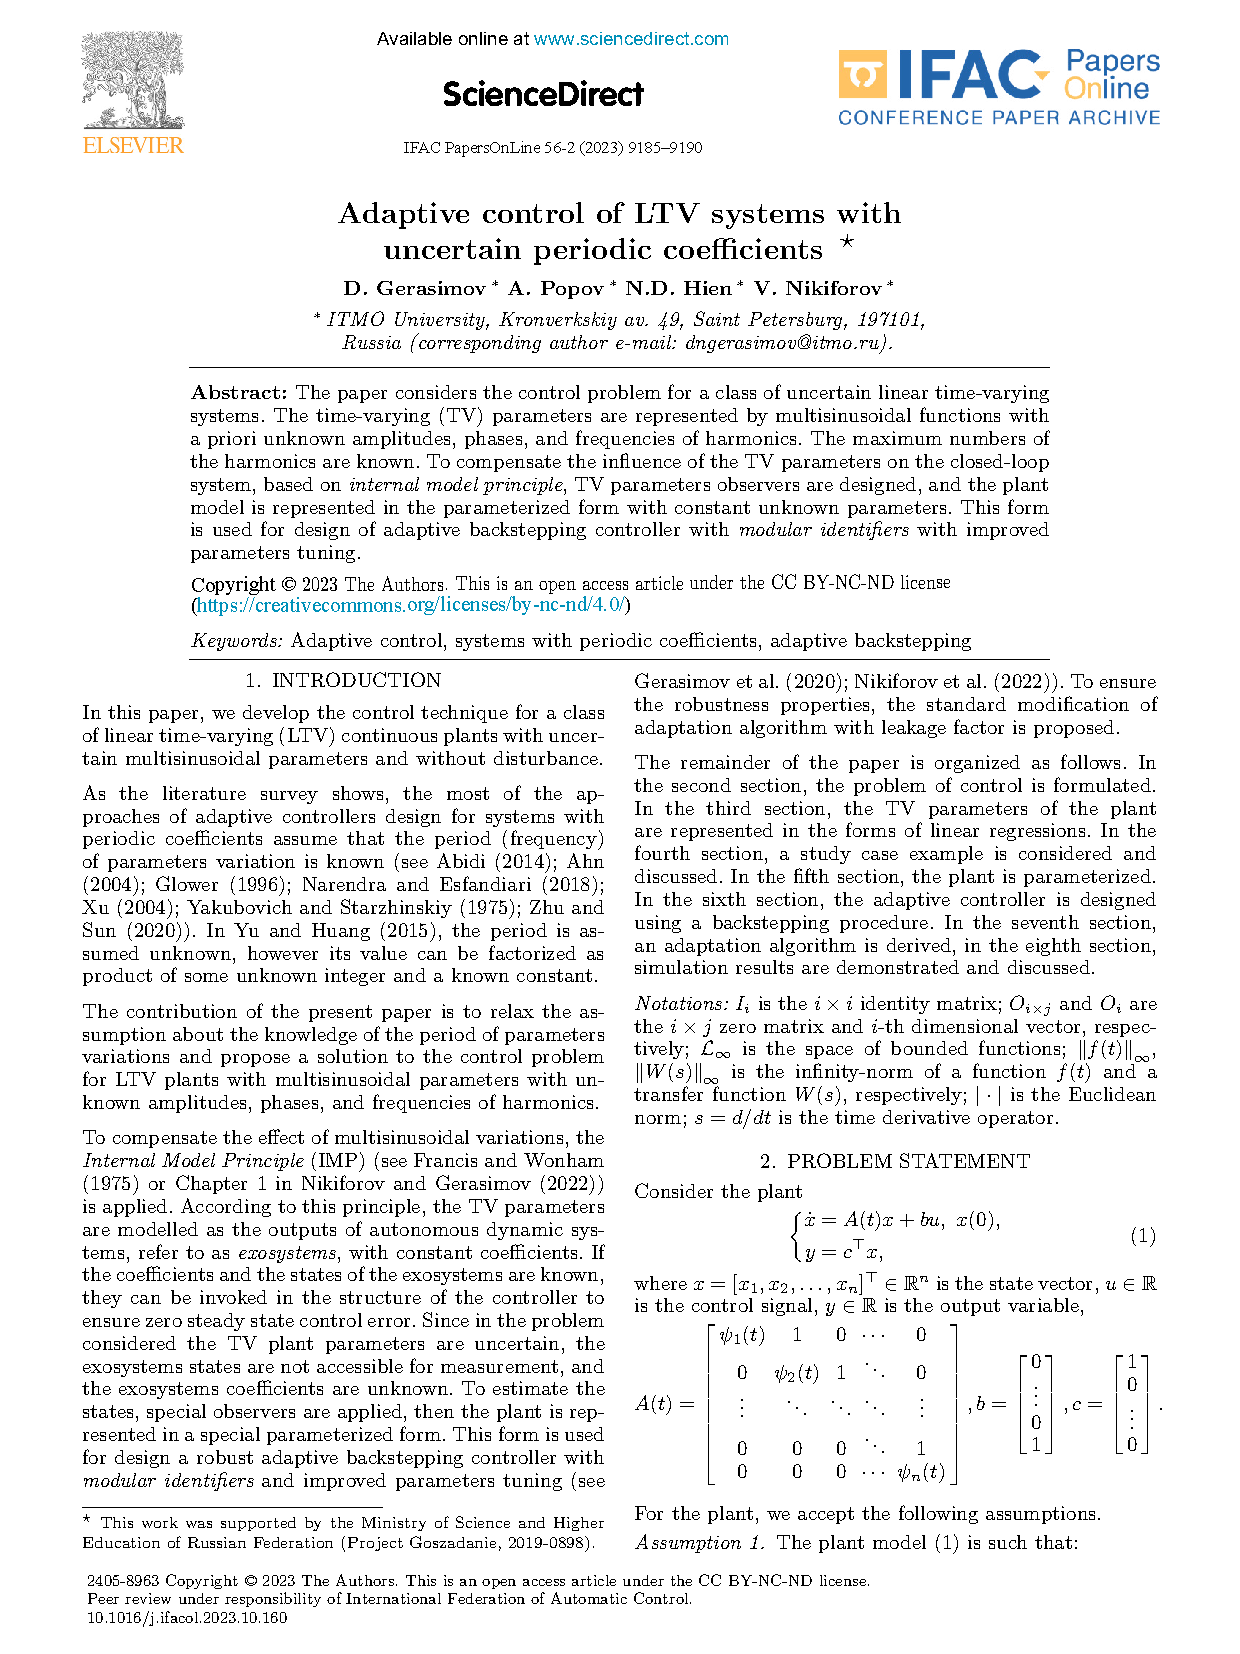
\includepdf[
pages={-},  %(include all pages) Selects pages to insert. pages=- will insert all pages of the document.
pagecommand={},  % to include global numbering
scale=0.9,  % to leave space for the global page numbers
%frame,  % Puts a frame around each logical page.
]{biblio/MyPublications/IFAC23_0519_FI-main.pdf}
 % тут же свои публикации
	\setcounter{totalappendix}{\value{chapter}} % Count the number of appendix

\end{document}
